\begin{mybilan}
	\begin{itemize}
		\item Un solide a un \kw{volume propre} et une \kw{forme propre}. Ses molécules sont \kw{organisées, fixes et proches les unes des autres}.
		
		\item Un \kw{liquide} a un \kw{volume propre mais pas de forme propre}. Ses particules sont \kw{proches les unes des autres mais peuvent se déplacer}. %les unes par rapport aux autres.
		
		\item Un gaz n'a \kw{ni forme propre ni volume propre}, il est compressible. Ses molécules sont \kw{éloignées les unes des autres et peuvent se déplacer}.
	\end{itemize}



\end{mybilan}

\begin{center}
	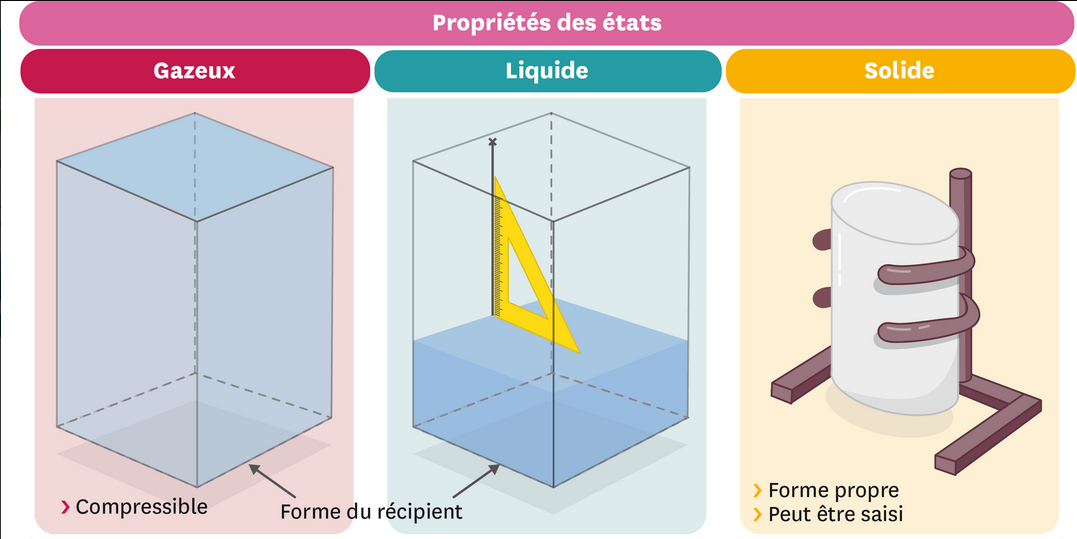
\includegraphics[scale=0.5]{img/etats}
\end{center}